\biohead{John Hill Munday}{c.~1900 at the Mendips.\cite{JHMmendips}}
\index{Munday, John Hill}

John Hill Munday was born on 6 July 1844 at 4 pm in Weymouth Street, Warminster, Wiltshire, England\cite{JHMtree, Census1861, JMHbirth} to William (\p{William_Munday}) and Mary (\p{Mary_Hill}). He had nine siblings: George Hill (1836--1862), Captain James William (1838--1875), Mary Elizabeth (1840--1849), Anna Maria (1841--1895), Sarah Adeline (1843--1924), Thomas Hill (1846--1862), Walter Edward (1847--1932), Nelson (1848--1886), and Louisa Fry (1851--1881).

John Munday was brought up by his maternal Aunt (Anna) Maria (n\'{e}e Hill) and Uncle \idx{Bruges Fry}. They lived at \idx{Beechcroft} (\f{Beechcroft}).

\begin{figure}
	\centering
	\includegraphics{photos/Beechcroft}
	\caption{``Beechcroft'', The Barrows, Cheddar, in 1934. This is where John Hill Munday lived as a child with his aunt and uncle Maria and Bruges Fry.\cite{BeechcroftPostcard}}
	\label{Beechcroft}
\end{figure}

His uncle was born in about 1810, son of Peter Fry of Compton Bishop, Axbridge; the Coroner and Registrar of the Somerset County Court.

In 1861 (aged 16) John Munday was still living with his aunt and uncle, at \emph{Hill House} in Silver Street, Cheddar,\cite{Census1861} 
and was working as a legal clerk for his uncle.\cite{Census1861}

In 1867 Bruges died at only 54 years of age;\cite{BrugesDeath} John Hill was 23, and moved to live with his parents.

In 1871, John Munday is listed as living with his parents and sister at 32 Middleton Road, Battersea and worked as a solicitor's morning clerk.\cite{JohnHillMunday1871} On 11 August 1876 he left on a long voyage to Natal, South Africa and wrote an extensive letter/diary about the journey---most of it was to do with life on board, and there is no record of what he did in Natal or why he had gone there: he returned by January 1877.

He married Catherine (n\'{e}e Aldridge, \p{Catherine_Aldridge}) on 8 April 1880 at Benhilton Church, Sutton, Croydon\cite{JHM-CA-marriage-announcement, JHMtree} and they had five children: Nora (\p{Nora_Katie_Munday}), Kathleen (\p{Kathleen_Munday}), Mildred (\p{Mildred_Mary_Munday}), Ralph (\p{Ralph_Munday}), and Margery (\p{Margery_Munday}).  They were living at 8 Shalston Villas, Ewell Road, Kingston upon Thames in 1881\cite{JohnHillMunday1881} and they then moved to live at the Mendips, Langley Avenue, Surbiton, (with six servants)  which was  a large house that he had had  built for the family [JohnHillMunday 1891].

He inherited Hill House, Paulton, Somerset (No.64 on the Paulton Tithe Map) from his Aunt Elizabeth Hill (widow of Thomas Ames Hill) when she died in 1901, which he sold to the tenant in 1902 (Walter Draper, market gardener) and he also inherited Holly Cottage, Paulton (sold in 1915 for two hundred pounds).

By 1901, they were still at the Mendips, with household staff of Cook, 2 parlourmaids, housemaid, domestic, kitchenmaid and coachman. The family moved on 3 May 1904 to Putney Hill, still with all five children at home (and three household staff).\cite{JohnHillMunday1911}

John Munday was a partner in the legal firm Ellis, Munday and Clarke, of College Hill Chambers, 23 College Hill, London\cite{HeaddingtonMannor} until he retired at the end of 1916[5].

The following comes from ``Opinions of the Lords of Appeal for Judgement in the Cause Prince Jefri Bolkiah v KPMG (A Firm)''\cite{JohnHillMundayJudgement}---

\begin{quotation}
\dots the decision of the Court of Appeal in Rakusen v. Ellis, Munday and Clarke [1912] 1 Ch. 831. The facts of that case were unusual. It concerned a small firm of solicitors with only two partners who carried on what amounted to separate practices, each with his own clients, without any knowledge of the other's clients and with the exclusive services of some of the clerks. The plaintiff consulted one of the partners in relation to a contentious matter. After he had terminated his retainer, the other partner, who had never met the plaintiff and was not aware that he had consulted his partner, was retained by the party opposite in the same matter. The judge granted an injunction to restrain the solicitor from acting. The Court of Appeal found that there was no risk of disclosure of confidential information and discharged the injunction. 
\end{quotation}

This was a landmark case.\cite{JohnHillMundayJudgement}

He died aged 73 on 15 January 1918,\cite{JHMdeath} committing suicide by jumping under a train at Surbiton or Putney Bridge Station, Surrey \cite{JohnHillMundaySuicide} and was cremated at Golders Green on 19 February 1918.

\begin{figure}
 \centering
 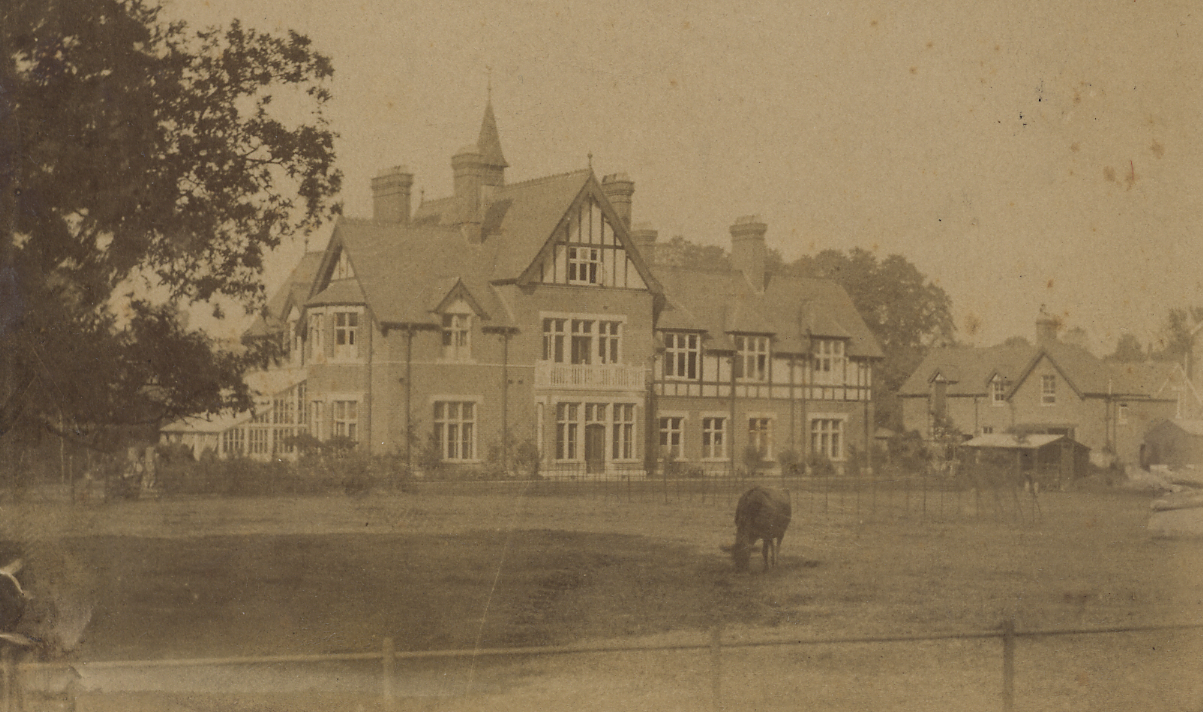
\includegraphics{photos/Mendips.png}
 \caption{The Mendips.}
\end{figure}

His obituary in the February 1918 edition of \emph{The Literary Guide} (the journal of the Rational Press Association) reads:

\begin{quotation}
\begin{center}
DIED,

On January 15, 1918,

JOHN HILL MUNDAY,

\emph{A Director of the Rationalist Press Association, Limited, for over fifteen years.}

Aged 73.
\end{center}

The death of Mr.\ J.\ H.\ Munday is a grevious loss to the Rationalist Press Association, of which he had been a Director since 1902, as well as its principal legal adviser. As senior partner in the firm of Messrs.\ Ellis, Munday, and Clarke, he was always busily employed, but he never failed to find opportunity to serve the R.~P.~A.~in any capacity; and he rarely missed attending the Board meetings, where his shrewd and common-sense judgement was always invaluable to his colleagues. His kind and genial disposition won him a host of friends, while his unimpeachable integrity invited a confidence and trust which he regarded as one of his richest possessions. In his home circle he was an ideal husband and a devoted father, and it can truly be said of him that he was beloved by all who knew him.

We first met Mr.\ Munday when the R.~P.~A.~was being established, and he assisted with other solicitors in drafting the Memoriandum and Articles of Association, without money and without price. Some five or six years ago he re-read the constitution in the light of later experience, and believing that the organization was destined to be one of Great Britain's foremost institutions, he suggested to the Board that he should at his leisure re-draft the Articles of Association, with the view of meeting any possible contingency which might arise. This necessitated much labour, including the convening of two meetings of the members of the Association; but the work was a labour of love to Mr.\ Munday, who presided at both gatherings, and explained the various alterations and additions with remarkable lucidity and to the complete satisfaction of all converned. The Articles, as they now stand, are not likely to require amendment within any measurable period, as they are adapted for well neigh every conceivable development of the work of the R.~P.~A.

Mr.\ Munday was a Life Member of the Association, and his name was seldom absent from any subscription list. His remains were cremated at Golders Green on the Saturday following his death, the service being conducted by Mr.~F.~J.~Gould, who delivered one of his characteristically impressive addresses. He leaves a widow, as well as a son and 4 daughters, to mourn his loss. We understand that in his will the R.~P.~A. is remembered.
\end{quotation}

The following funeral oration was given by Frederick Gould:\cite{JohnHillMundayFuneral}
 
\begin{quotation}
'Our dear friend, John Hill Munday, had, many years ago, courageously and decisively made up his mind as to his relations with his fellow-man and with nature at large. Towards his fellow-men his attitude was that of duty and honour. Towards nature his attitude was one of study and reasoned obedience, without any attempt to penetrate to supernatural secrets, or to spend golden time in discovering a world beyond death. In other words, he was both a good citizen and a staunch Rationalist. Such was his record, honest and clear, when he died at the age of 73. His memory is honoured by wife, son and daughters, and by his comrades in the struggle - the victorious struggle - for liberty and progress of thought. When, nearly twenty years ago, a small band of us laid the foundations of the Rationalist Press Association, our friend not only gave his sympathy to this effort on behalf of intellectual light for England and the world; he rendered substantial aid in drawing up the Articles of the new Association. For it was important, besides taking up the enterprise for freedom of the mind with enthusiasm, and to refine and state its objects with plainness, with precision, with business-like and prudent word and phrase so as to give confidence to supporters as well as candid and unmistakeable notice to the public. Trained and accustomed to the practice of law, our friend proved that he was both a good solicitor and and earnest disciple of Reason and Humanism. He took a seat willingly at the Board of the Association, and his fellow Directors found him, from the beginning and all the time, a most useful and competent colleague; not fond of much speaking, but attending with regularity and devoting careful consideration to all plans and proposals. Seven years ago, his keen legal eye detected certain points in the R.P.A. articles that needed improvement and safe-guarding. Like a man who schemes a building, and desires to lay its stones and beams truly and well, he framed a new statement, met his colleagues in many consultations, presided, discussed, persuaded, persevered, and so at length satisfied himself and his friends that the Association was solidly established and its aims more efficiently promoted. The work of months was tedious, but all was done with good heart and a valiant purpose. In matters of political and other opinions, he was for his own part firm and consistent; but towards those who differed, even towards the odd and eccentric, he was good-naturedly tolerant. It was therefor most natural that his colleagues should feel a very kindly attachment for him. On his retirement from partnership in his law-firm the R.P.A. Board assured him of their cordial respect. His reply intimated that, in co-operating for the spread of Rationalism (and hence for the welfare of mankind) he had spent the happiest hours of his life. It was, indeed, that fruitful kind of happiness which was good for the man himself, and good for world-wide humanity. And here may be noted two things in our friends' field of interest. He was always glad to hear of the extended circulation of books that aimed at the moral training of the young on humanist and rational lines. And he was specially active in the dispatch of our literature to soldiers engaged in the war, in camp or at the front; and may have been the evidences that such gifts were appreciated.

On the hearts of his wife and children is graven the recollection of his constant and tender thoughtfulness in the relationships and experiences of the home. Whatever may have been his sense of physical failure in the latter days, his master motive was to arrange affairs, to guard against discomforts, to provide for the future - in a word, to do all that a kind ingenuity and practical sense could suggest to ensure the peace and solace of those he loved, and assistance to the public cause for which he had so untiringly laboured. A man of absolute integrity in his business, a very loyal friend, a sure keeper of the plighted word, he was of simple taste and habit; and he desired this simplicity to mark the last rites. Hence we see here no crowding of memorial flowers. But there is at least one flower that we offer, and one that he would have thought of with a smile of gratitude - the flower of respect and hommage for a life of usefulness , of steady and brave conviction, of fidelity to an unpopular cause, of domestic affection and of generosity towards his fellow men."

Frederick J. Gould \\
Saturday 19th February 1918
\end{quotation}

The probate notice read: ``MUNDAY John Hill of Cedar Lodge 21 St Johns Road, Putney Hill, Surrey died 15 January 1918 at or near St Thomas Hospital Surrey. Probate London 12 March to the Public Trustee. Effects \pounds18,041.19s.1d (Will registered 1 December 1916).\cite{NationalProbateCalendar}
